\documentclass[paper=a4, fontsize=11pt]{scrartcl}
\usepackage{silence}
\WarningFilter{scrartcl}{Usage of package `fancyhdr'}
\usepackage{cite}
\usepackage[T1]{fontenc}
\usepackage{fourier}

\usepackage[english]{babel}                             % English language/hyphenation
\usepackage[protrusion=true,expansion=true]{microtype}  
\usepackage{amsmath,amsfonts,amsthm} % Math packages
\usepackage[pdftex]{graphicx} 
\usepackage{url}
\usepackage[section]{placeins}

%%% Unicode character declaration


%%% Custom sectioning
\usepackage{sectsty}
\allsectionsfont{\centering \normalfont\scshape}
\usepackage{color}
\usepackage{color,soul}

%%% Custom headers/footers (fancyhdr package)
\usepackage{fancyhdr}
\pagestyle{fancyplain}
\fancyhead{}                      % No page header
\fancyfoot[L]{}                     % Empty 
\fancyfoot[C]{}                     % Empty
\fancyfoot[R]{\thepage}                 % Pagenumbering
\renewcommand{\headrulewidth}{0pt}      % Remove header underlines
\renewcommand{\footrulewidth}{0pt}        % Remove footer underlines
\setlength{\headheight}{13.6pt}


%%% Equation and float numbering
\numberwithin{equation}{section}    % Equationnumbering: section.eq#
\numberwithin{figure}{section}      % Figurenumbering: section.fig#
\numberwithin{table}{section}       % Tablenumbering: section.tab#


%%% Maketitle metadata
\newcommand{\horrule}[1]{\rule{\linewidth}{#1}}   % Horizontal rule

\title{
    %\vspace{-1in}  
    \usefont{OT1}{bch}{b}{n}
    \normalfont \normalsize \textsc{Carnegie Mellon University - Computational Biology Department} \\ [25pt]
    \today \\
    \horrule{0.5pt} \\[0.4cm]
    \huge Predicting Pseudouridylation of Individual RNA Bases Using Machine Learning\\
    \horrule{2pt} \\[0.5cm]
}
\author{
  Christine Baek\\
  \normalsize\texttt{christib@andrew.cmu.edu}
  \and
  Kevin Chon\\
  \normalsize\texttt{khchon@andrew.cmu.edu}
  \and
  Deepank Korandla\\
  \normalsize\texttt{dkorandl@andrew.cmu.edu}
   \and
  Tianqi Tang\\
  \normalsize\texttt{tianqit1@andrew.cmu.edu}
  \date{}
}
\date{}


\newcommand{\TODO}[1]{\textcolor{red}{\textbf{TODO: } #1}}

%%% Equation and float numbering
\numberwithin{equation}{section}    % Equationnumbering: section.eq#
\numberwithin{figure}{section}      % Figurenumbering: section.fig#
\numberwithin{table}{section}       % Tablenumbering: section.tab#
\usepackage[T1]{fontenc}
\usepackage[utf8]{inputenc}
\usepackage{textcomp}
\usepackage{tabularx,ragged2e,booktabs,caption}
\newcolumntype{C}[1]{>{\Centering}m{#1}}
\renewcommand\tabularxcolumn[1]{C{#1}}



%%% Begin document
\begin{document}

\maketitle

\begin{abstract}
\TODO{CHRISTINE abstract here. CB will complete this section after all other sections are written}

We have built a software that predicts the probability of each site of input RNA sequence being pseudoUracil. 
\end{abstract}


\section{Introduction}

\TODO{DEEPANK. 3 sections minimum covering 1) RNA modification - what is it, biological significance. 2) PseudoUracil - what is it, maybe include figure of pseudouracil 3) What has been done with PseudoUracil research. DO NOT FORGET TO CITE.}

example for Deepank : 

This is how you cite stuff ~\cite{schwartz}.



%%% Methods

\section{Methods}


The goal of this project is that we have to build a per-base/position predictor of pseudouridylation probability. Main challenge were small amount of related previous work whose models which could be used as reference, and extremely limited labeled data to train with. Our data represents both \textit{breadth and depth} in that the data represents intra-species, intra-gene, and inter-species diversity of pseudouracil. We have built models using different combinations of data to build a final model that is generalizable to different species and genes. The final software takes in standard bioinformatics data format such as \texttt{.fasta} or \texttt{.mfa} and outputs the probability of each base being pseuouracil. 


\subsection{Relevant Domain Knowledge}

Previous work on RNA modification suggest that such modifications are sequence-dependent. Also, the secondary RNA structure is known to be important for various biological function. We worked with all publicly available RNA pseudouridylation data and for these, both the raw sequence and secondary structure were used as features. We chose two popular machine learning approaches (random forest and SVM) for our learning model, given their popularity and known robustness when analyzing biological data. 

\subsection{Data}

This section discusses the type of data and their source, how they were processed and the features chosen for our models.

\subsubsection{Data Collection}

Total of 3 data sets were used. 

\begin{enumerate}
	\item \textit{homo sapiens} chromosome rRNA ~\cite{schwartz} - this dataset represents intra-genome, inter-gene data (breadth-focused - same species, varied genes)
	\item \textit{homo sapiens} rRNA ~\cite{carlile} - this dataset represents intra-genome, intra-gene data (depth-focused)
	\item Aligned rRNA from following organisms ~\cite{modomics} - this dataset represents inter-genome, intra-gene data (breadth-focused - varied species, same gene)
    	\begin{itemize}
        \item \textit{Escherichia coli}
        \item \textit{Bacillus subtilis}
        \item \textit{Clostridium acetobutylicum}
        \item \textit{Thermotoga maritima}
        \item \textit{Thermus thermophilus}
        \item \textit{Pyrococcus abyssi}
        \item \textit{Sulfolobus solfataricus}
        \item \textit{Arabidopsis thaliana}
        \item \textit{Homo sapiens}
        \item \textit{Saccharomyces cerevisiae}
        \end{itemize}
\end{enumerate}

Dataset 2 functions as the common ground, or the connection between dataset 1 and 3. 

\subsubsection{Data Processing}

\TODO{CHRISTINE : obtaining the actual data, modifying it}

\subsection{Feature Selection \& Engineering}

\TODO{CHRISTINE :  GC content, sliding window}

While it is possible that both direct neighboring sequences and potentially far sequences (in the form of secondary structure/hairpin) may have an impact on pseudouridylation, that would also indicate that the sequence 
Why delta G was rejected. 

\TODO{TIANQI : discuss stuff like vienna/RNA fold}




\subsection{Machine Learning Algorithm}

The most popular strategy in applying machine learning currently is to attempt multiple strategies, and select for the best performing models. We chose SVM and Random Forest for their established performance and popularity for medical and biological data. 

\subsubsection{SVM}

\TODO{TIANQI - talk about why you picked SVM, what SVM is, and some settings you may be using and why.}

There are a numbers of different classifiers that can help solving the problem, e.g. logistic regression, Naive Bayes classifier, neural network, random forest and support vector machine(SVM). Among these classifiers SVM has a great balance between performance and computational complexity, so we are using support vector machine with radial basis kernel in this project. Support vector machine is a supervised learning algorithm whose goal is to find the hyperplane that has the largest separation between two classes. 

When the training samples are not linearly separable, we can use two techniques, soft margin and kernel. Soft margin allows misclassification in training step. Kernel projects the samples into a different space, making the samples to be linear separable. For example, in a two dimensional space two sets of data points locate on two different circles, both have the origin as center, and have radius $r_1$ and $r_2$. These data points are not separable by a straight line, but after projection $\phi(\boldsymbol{x})=x_1^2+x_2^2$, the data points can be separated by a line. In practice people usually use the product of the projection of two points, denoted as $\boldsymbol{K}(\boldsymbol{x},\boldsymbol{x'})=\phi(\boldsymbol{x})\phi(\boldsymbol{x'})$.

In this project we used radial basis function(RBF) kernel. The kernel function of RBF is $\boldsymbol{K}(\boldsymbol{x},\boldsymbol{x'})=\exp(-\frac{\|\boldsymbol{x}-\boldsymbol{x'}\|_2^2}{2\sigma^2})$, $\sigma^2$ is the parameter given by user. Under Taylor series expansion it is a polynomial function with infinite order, so it can project the samples into a infinity dimension space and can fits any shape of sample distribution.



\subsubsection{Random Forest}

\TODO{KEVIN - talk about why you picked SVM, what SVM is, and some settings you may be using and why.}

%%% Results

\section{Results}

\subsection{SVM Results}

\TODO{TIANQI - discuss the results, and provide the table of performances where columns are input data type, and rows are various parameters used. Please use some form of heat map for the resulting table. I recommend matlab. Kevin \& Tianqi - talk to each other so that the two tables look simliar (colorscheme, format, etc.) for uniformity}

% Table generated by Excel2LaTeX from sheet 'Sheet1'
\begin{table}[htbp]
  \centering
  \caption{Add caption}
    \begin{tabular}{cccc}
    Window size & f1\_weighted & precision & recall \\
    3     & 90.64\% & 99.29\% & 84.12\% \\
    5     & 95.08\% & 99.09\% & 91.84\% \\
    7     & 96.70\% & 98.83\% & 94.84\% \\
    9     & 97.99\% & 98.75\% & 97.35\% \\
    11    & 98.51\% & 98.58\% & 98.46\% \\
    13    & 98.62\% & 98.50\% & 98.75\% \\
    15    & 98.73\% & 98.50\% & 98.96\% \\
    17    & 98.82\% & 98.59\% & 99.09\% \\
    19    & 98.82\% & 98.51\% & 99.14\% \\
    21    & 98.83\% & 98.51\% & 99.15\% \\
    23    & 98.86\% & 98.51\% & 99.22\% \\
    25    & 98.86\% & 98.51\% & 99.21\% \\
    27    & 98.87\% & 98.51\% & 99.24\% \\
    29    & 98.87\% & 98.51\% & 99.24\% \\
    31    & 98.88\% & 98.51\% & 99.25\% \\
    33    & 98.88\% & 98.51\% & 99.25\% \\
    35    & 98.88\% & 98.51\% & 99.25\% \\
    37    & 98.88\% & 98.51\% & 99.25\% \\
    39    & 98.88\% & 98.51\% & 99.25\% \\
    \end{tabular}%
  \label{tab:addlabel}%
\end{table}%

\begin{center}
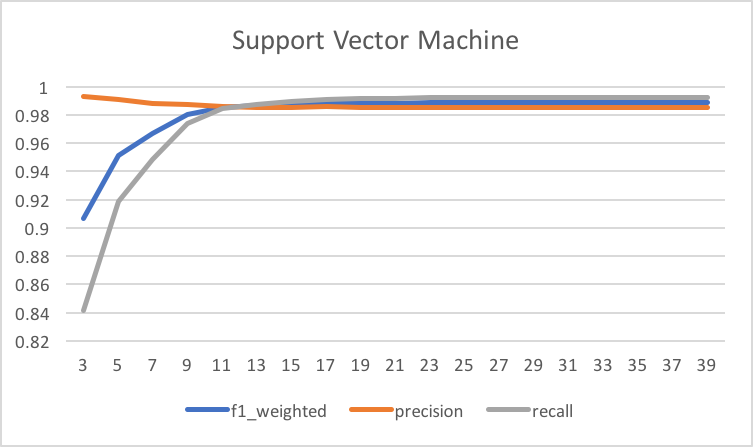
\includegraphics{SVM_f1}
\end{center}
\FloatBarrier

\subsection{Random Forest Results}

\TODO{KEVIN - discuss the results, and provide the table of performances where columns are input data type, and rows are various parameters used. Please use some form of heat map for the resulting table. I recommend matlab. Kevin \& Tianqi - talk to each other so that the two tables look simliar (colorscheme, format, etc.) for uniformity}


\section{Evaluation of Other Teams' Work}

\subsection{Team B}

\subsubsection{Issues during Installation}
- how easy was it to install?

Would be better if support both Python 2 and 3 support, or indicate which Python 2 only packages are used.
Not easy to install and use because of tons of prerequisite softwares.

\subsubsection{Model Design}
- does design make sense? do you understand what the design is?

The design seems to be clear in terms of how a machine learning algorithm is being trained and tested, even though there are references to several other libraries and how to use them.


\subsubsection{Model Performance}
- does it seem to perform well ?

Seems good

\subsubsection{Potential Improvements}
- clear interface/definitions ? what could be done better?

Just keep the least necessary files when distributing your software. A pipeline means user can do the whole things with one command, not download a bunch of prerequisite softwares, generate the data you need, to serve your software.  People will also not going to train the model themselves, what they need is a pre-trained model. Just keep users away from those verbose information if they do not need it.

\subsection{Team C}

\subsubsection{Issues during Installation}
- how easy was it to install?

- If asking people to download stuff, either include the commands OR direct link at the minimum. 

There is no context for what the input files should contain (at least in the description section). There is no warning that pysam is not supported by Windows. No sample files input provided. This means I cannot skip the alignment step and move on to the detection step. For the alignment step, I am not sure where I am supposed to get a fastq file with sequence reads, and the group expects me to download the entire human genome (no reference site is provided either). The usage section could have better step-by-step directions. It is not immediately evident that the "Alignment of Reads" section can be skipped.

\subsubsection{Model Design}
- does design make sense? do you understand what the design is?

Seems to align the input sequence to the model genome using BowTie2 and SamTools, which then can be put through the pre-trained classifier, outputting windows of m1a modifications. 


\subsubsection{Model Performance}
- does it seem to perform well ?

It seems that the model is trained on only human... ? or that's my impression based on the readme. 

\subsubsection{Potential Improvements}
- clear interface/definitions ? what could be done better?

\begin{itemize}
	\item Include the location of m1a on the reference genome instead of just the window
    \item only humans?
    \item Seriously? You want ME to download the reference genome? How about at least including a direct link
    
\end{itemize}


\section{Future Directions}

\TODO{Christine, but get input from others}
- more data
- try more models
- 

%%% Conclusion

\section{Conclusion}

\TODO{CHRISTINE - done after all other sections are filled out}
- our model works reasonably well
- RNA hairpin didn't work



%%% Bibliography


\begin{thebibliography}{1}

% use the following format for each new citation. Items that need to be modified are capitalized
\bibitem{example}
AUTHOR1, AUTHOR2, et al.
\hskip 1em plus 0.5em minus 0.4em\relax 
\emph{TITLE}  
\hskip 1em plus 0.5em minus 0.4em\relax 
http://LINK, 
DATE OF PUBLICATION



\bibitem{schwartz}
Schraga Schwartz and Douglas A. Bernstein and Maxwell R. Mumbach and Marko Jovanovic and Rebecca H. Herbst and Brian X. Leon-Ricardo and Jesse M. Engreitz and Mitchell Guttman and Rahul Satija and Eric S. Lander and Gerald Fink and Aviv Regev
\hskip 1em plus 0.5em minus 0.4em\relax 
\emph{Transcriptome-wide Mapping Reveals Widespread Dynamic-Regulated Pseudouridylation of ncRNA and mRNA}  
\hskip 1em plus 0.5em minus 0.4em\relax 
http://doi.org/10.1016/j.cell.2014.08.028, 
2014

\bibitem{modomics}
International Institute of Molecular and Cell Biology in Warsaw
\hskip 1em plus 0.5em minus 0.4em\relax 
\emph{RNA sequences with modifications}  
\hskip 1em plus 0.5em minus 0.4em\relax 
http://modomics.genesilico.pl/sequences/list/
accessed April 1, 2017

\bibitem{carlile}
Thomas M. Carlile, Maria F. Rojas-Duran, Boris Zinshteyn, Hakyung Shin, Kristen M. Bartoli, and Wendy V. Gilbert
\hskip 1em plus 0.5em minus 0.4em\relax 
\emph{Pseudouridine profiling reveals regulated mRNA pseudouridylation in yeast and human cells}  
\hskip 1em plus 0.5em minus 0.4em\relax 
https://www.ncbi.nlm.nih.gov/pmc/articles/PMC4224642/
DATE OF PUBLICATION

\end{thebibliography}

\end{document}